\documentclass[12pt,a4paper]{report}
\usepackage[utf8]{inputenc}
\usepackage[T1]{fontenc}
\usepackage{mathptmx} % Times New Roman benzeri font
\usepackage[turkish]{babel}
\usepackage{graphicx}
\usepackage{hyperref}
\usepackage{listings}
\usepackage{xcolor}
\usepackage{geometry}
\usepackage{booktabs}
\usepackage{longtable}
\usepackage{fancyhdr}
\usepackage{titlesec}
\usepackage{float}
\usepackage{array}
\usepackage{amsmath}
\usepackage{caption}
\usepackage{subcaption}
\usepackage{tikz}
\usetikzlibrary{shapes.geometric, arrows, positioning, calc, babel} % babel kütüphanesi eklendi

% Sayfa Yapısı
\geometry{
    left=30mm,
    right=25mm,
    top=30mm,
    bottom=25mm
}

% Link Ayarları
\hypersetup{
    colorlinks=true,
    linkcolor=black,
    filecolor=magenta,      
    urlcolor=blue,
    pdftitle={Bitirme Projesi Final Raporu - Bi Dakika},
    pdfauthor={Nuh Demir},
    pdfpagemode=FullScreen,
}

% Kod Bloğu Renkleri ve Ayarları
\definecolor{codegreen}{rgb}{0,0.6,0}
\definecolor{codegray}{rgb}{0.5,0.5,0.5}
\definecolor{codepurple}{rgb}{0.58,0,0.82}
\definecolor{backcolour}{rgb}{0.96,0.96,0.96}

\lstdefinestyle{mystyle}{
    backgroundcolor=\color{backcolour},   
    commentstyle=\color{codegreen},
    keywordstyle=\color{magenta},
    numberstyle=\tiny\color{codegray},
    stringstyle=\color{codepurple},
    basicstyle=\ttfamily\footnotesize,
    breakatwhitespace=false,         
    breaklines=true,                 
    captionpos=b,                    
    keepspaces=true,                 
    numbers=left,                    
    numbersep=5pt,                  
    showspaces=false,                
    showstringspaces=false,
    showtabs=false,                  
    tabsize=2,
    frame=single
}
\lstset{style=mystyle}

% Başlık Formatlama
\titleformat{\chapter}[display]
  {\normalfont\huge\bfseries\centering}{\chaptertitlename\ \thechapter}{20pt}{\Huge}
\titlespacing*{\chapter}{0pt}{0pt}{40pt}

% Üst ve Alt Bilgi
\pagestyle{fancy}
\fancyhf{}
\fancyhead[L]{\slshape \leftmark}
\fancyhead[R]{\thepage}
\renewcommand{\chaptermark}[1]{\markboth{#1}{}}

\begin{document}

% -------------------------------------------------------------------
% KAPAK SAYFASI
% -------------------------------------------------------------------
\begin{titlepage}
    \begin{center}
        \vspace*{0.5cm}
        \Large\textbf{T.C.}\\
        \Large\textbf{BARTIN ÜNİVERSİTESİ}\\
        \large\textbf{FEN FAKÜLTESİ}\\
        \large\textbf{BİLGİSAYAR TEKNOLOJİSİ VE BİLİŞİM SİSTEMLERİ}
        
        \vspace{4cm}
        
        \Huge \textbf{Bİ DAKİKA}\\
        \Large \textbf{YENİ NESİL MİKRO-ÖĞRENME TABANLI}\\
        \Large \textbf{DİL EĞİTİM PLATFORMU}
        
        \vspace{3cm}
        
        \Large \textbf{BİTİRME PROJESİ FİNAL RAPORU}
        
        \vspace{3cm}
        
        \begin{tabular}{ll}
            \textbf{Hazırlayan:} & Nuh DEMİR \\
            \textbf{Öğrenci No:} & 22010708018
        \end{tabular}
        
        \vfill
        
        \Large \textbf{BARTIN, 2026}
        
    \end{center}
\end{titlepage}

% -------------------------------------------------------------------
% ÖZET
% -------------------------------------------------------------------
\chapter*{Özet}
\addcontentsline{toc}{chapter}{Özet}

Bu bitirme projesi kapsamında geliştirilen \textbf{"Bi Dakika"}, geleneksel dil öğrenme yöntemlerinin hantallığını ve motivasyon eksikliğini ortadan kaldırmayı hedefleyen, mikro-öğrenme (micro-learning) prensiplerine dayalı mobil bir uygulamadır. Günümüzün hızla değişen dünyasında, kullanıcıların uzun süreli dikkat sürelerine sahip olmaması gerçeğinden yola çıkılarak tasarlanan bu platform, günde sadece birkaç dakika ayrılarak dil yetkinliğinin artırılmasını hedefler.

Sistem mimarisi, milyonlarca eşzamanlı kullanıcıyı destekleyebilecek ölçeklenebilirlikte tasarlanmıştır. Backend tarafında NestJS framework'ü, veri tutarlılığı ve performans için PostgreSQL veritabanı ile birlikte kullanılmıştır. Veri erişim katmanında Prisma ORM, karmaşık sorguların tip güvenli bir şekilde yönetilmesini sağlar. Yüksek trafikli senaryolar için "Event-Driven" mimari benimsenmiş, Redis ve BullMQ teknolojileri ile asenkron işlem kuyrukları oluşturulmuştur.

Ön yüzde kullanıcı deneyimini (UX) maksimize etmek amacıyla React Native ve Expo kullanılarak iOS ve Android platformlarında çalışan cross-platform bir uygulama geliştirilmiştir. Uygulama, Aralıklı Tekrar Sistemi (Spaced Repetition System - SRS) gibi gelişmiş algoritmaları, lig sistemi ve ödül mekanizmaları gibi oyunlaştırma (gamification) öğeleriyle harmanlayarak kullanıcı bağlığını (retention) en üst düzeye çıkarmaktadır.

\textbf{Anahtar Kelimeler:} Mobil Öğrenme, Oyunlaştırma, NestJS, React Native, PostgreSQL, Mikro-Öğrenme, SRS.

\newpage

% -------------------------------------------------------------------
% ABSTRACT
% -------------------------------------------------------------------
\chapter*{Abstract}
\addcontentsline{toc}{chapter}{Abstract}

Developed within the scope of this graduation project, \textbf{"Bi Dakika" (One Minute)} is a mobile application based on micro-learning principles, aimed at eliminating the clumsiness and lack of motivation inherent in traditional language learning methods. Designed with the reality that users in today's fast-changing world have short attention spans, this platform aims to increase language proficiency by dedicating just a few minutes a day.

The system architecture is designed to support millions of concurrent users. On the backend, the NestJS framework is utilized alongside a PostgreSQL database to ensure data consistency and performance. Prisma ORM in the data access layer ensures type-safe management of complex queries. An "Event-Driven" architecture has been adopted for high-traffic scenarios, establishing asynchronous job queues with Redis and BullMQ technologies.

On the frontend, a cross-platform application running on iOS and Android has been developed using React Native and Expo to maximize User Experience (UX). The application blends advanced algorithms like the Spaced Repetition System (SRS) with gamification elements such as league systems and reward mechanisms, thereby maximizing user retention.

\textbf{Keywords:} Mobile Learning, Gamification, NestJS, React Native, PostgreSQL, Micro-Learning, SRS.

\newpage

% -------------------------------------------------------------------
% İÇİNDEKİLER
% -------------------------------------------------------------------
\tableofcontents
\listoftables
\listoffigures
\newpage

% -------------------------------------------------------------------
% BÖLÜM 1: GİRİŞ
% -------------------------------------------------------------------
\chapter{Giriş}

\section{Projenin Tanımı ve Kapsamı}
\textbf{Bi Dakika}, kullanıcıların yoğun günlük tempoları arasında dil öğrenmeye ayırabilecekleri kısa zaman dilimlerini en verimli şekilde değerlendirmelerini sağlayan akıllı bir eğitim asistanıdır. "Bir dakika" metaforu, öğrenme eyleminin başlatılması için gereken zihinsel bariyeri düşürmeyi hedefler. Proje, sadece bir mobil uygulama (Frontend) değil, aynı zamanda bu uygulamayı besleyen, kullanıcı verilerini analiz eden ve kişiselleştirilmiş içerik sunan güçlü bir Backend servisini de kapsamaktadır.

\section{Problem Bildirimi}
Mevcut dil öğrenme ekosisteminde gözlemlenen temel problemler şunlardır:
\begin{enumerate}
    \item \textbf{Zaman Yönetimi Sorunu:} Geleneksel kurslar ve uzun video içerikler, modern kullanıcının yaşam stiline uyum sağlayamamaktadır.
    \item \textbf{Motivasyon Kaybı:} Uzun süren ve hemen ödül vermeyen öğrenme süreçleri, kullanıcıların %80'inin ilk ayda eğitimi bırakmasına ("Churn") neden olmaktadır.
    \item \textbf{Teknik Yetersizlikler:} Piyasadaki birçok uygulama, yüksek kullanıcı sayılarına ulaştığında performans sorunları yaşamakta ve çevrimdışı (offline) kullanım desteği sunmamaktadır.
\end{enumerate}

\section{Çözüm Önerisi: Bi Dakika Yaklaşımı}
Bi Dakika, eğitim materyallerini atomik parçalara ayırarak (\textit{bite-sized content}) sunar. Her bir egzersiz veya ders, otobüs beklerken veya kahve molasında tamamlanabilecek kadar kısadır. Ancak arka planda çalışan yapay zeka destekli algoritmalar, bu kısa etkileşimlerin uzun vadeli belleğe aktarılmasını garanti eder.

\section{Özgün Değer (Unique Value Proposition)}
Projenin rakiplerinden ayrılan en önemli özelliği, \textbf{"Teknik Derinlik ile Pedagojik Basitliğin Sentezi"}dir. Arayüz son derece basit tutulurken, arka planda çalışan sistem; finansal sistemlerde kullanılan "Transaction" güvenliğini, büyük veri sistemlerinde kullanılan "Partitioning" tekniklerini ve nörobilimsel öğrenme modellerini (SM-2) kullanır.

% -------------------------------------------------------------------
% BÖLÜM 2: LİTERATÜR VE YÖNTEM
% -------------------------------------------------------------------
\chapter{Literatür Özeti ve Metodoloji}

\section{Mikro-Öğrenme ve Oyunlaştırma}
Literatürdeki çalışmalar, öğrenme materyallerinin küçük parçalara bölünmesinin bilişsel yükü (cognitive load) azalttığını göstermektedir (Miller, 1956). Ayrıca, oyunlaştırma dinamiklerinin (Deterding et al., 2011) dopamin salgılanmasını tetikleyerek öğrenme isteğini artırdığı kanıtlanmıştır. Bi Dakika, bu iki akademik yaklaşımı teknik bir ürüne dönüştürmüştür.

\section{Yazılım Geliştirme Metodolojisi}
Proje geliştirme sürecinde \textbf{30 Fazlı Artımlı Geliştirme (Incremental Development)} modeli izlenmiştir. Her faz, test edilebilir bir ürün parçası (increment) ortaya koymuştur.
\begin{itemize}
    \item \textbf{Faz 1-5:} Altyapı kurulumu ve veritabanı mimarisi.
    \item \textbf{Faz 6-15:} Çekirdek motor (Core Engine) geliştirimi.
    \item \textbf{Faz 16-25:} Sosyal katman ve ekonomi modülleri.
    \item \textbf{Faz 26-30:} Performans optimizasyonu ve ölçekleme.
\end{itemize}

\section{Kullanılan Teknolojiler ve Gerekçeleri}

\begin{table}[H]
    \centering
    \caption{Proje Teknoloji Yığını}
    \label{tab:tech-stack}
    \begin{tabular}{|p{4cm}|p{4cm}|p{6cm}|}
        \hline
        \textbf{Katman} & \textbf{Teknoloji} & \textbf{Seçim Gerekçesi} \\
        \hline
        Backend Framework & NestJS & Modüler mimari, TypeScript desteği ve Dependency Injection yeteneği. \\
        \hline
        Veritabanı & PostgreSQL 16+ & JSONB desteği, Partitioning yeteneği ve ACIS transaction güvenliği. \\
        \hline
        ORM & Prisma & Tip güvenliği (Type-safety) ve güçlü şema migrasyon araçları. \\
        \hline
        Mobil Framework & React Native (Expo) & Tek kod tabanı ile hem iOS hem Android çıktısı alabilme hızı. \\
        \hline
        Bağlantı Havuzu & PgBouncer & Serverless ve Container ortamlarında bağlantı limitlerini yönetebilme. \\
        \hline
        Kuyruk Sistemi & Redis \& BullMQ & Yüksek hacimli yazma işlemlerini asenkronize etme. \\
        \hline
    \end{tabular}
\end{table}

% -------------------------------------------------------------------
% BÖLÜM 3: SİSTEM MİMARİSİ VE ALGORİTMİK ALTYAPI
% -------------------------------------------------------------------
\chapter{Sistem Mimarisi ve Algoritmik Altyapı}

\section{Mimari Prensipler ve Tasarım}
Bi Dakika platformu, \textbf{"Event-Driven Microservices-Ready Monolith"} (Olay Tabanlı Mikroservislere Hazır Monolit) mimari prensibiyle tasarlanmıştır. Bu strateji, başlangıçta monolitik yapının sağladığı geliştirme hızını ve veri bütünlüğünü sunarken, sistem büyüdükçe parçalanabilir, gevşek bağlı (loosely-coupled) bir yapı kurmayı hedefler.

\subsection{Sistem Bileşen Diyagramı}
Sistemin veri akış mimarisi, yüksek trafik ve eşzamanlı istekleri yönetmek üzere tasarlanmış katmanlardan oluşur. Aşağıdaki şekilde sistemin genel topolojisi görülmektedir:

\begin{figure}[H]
\centering
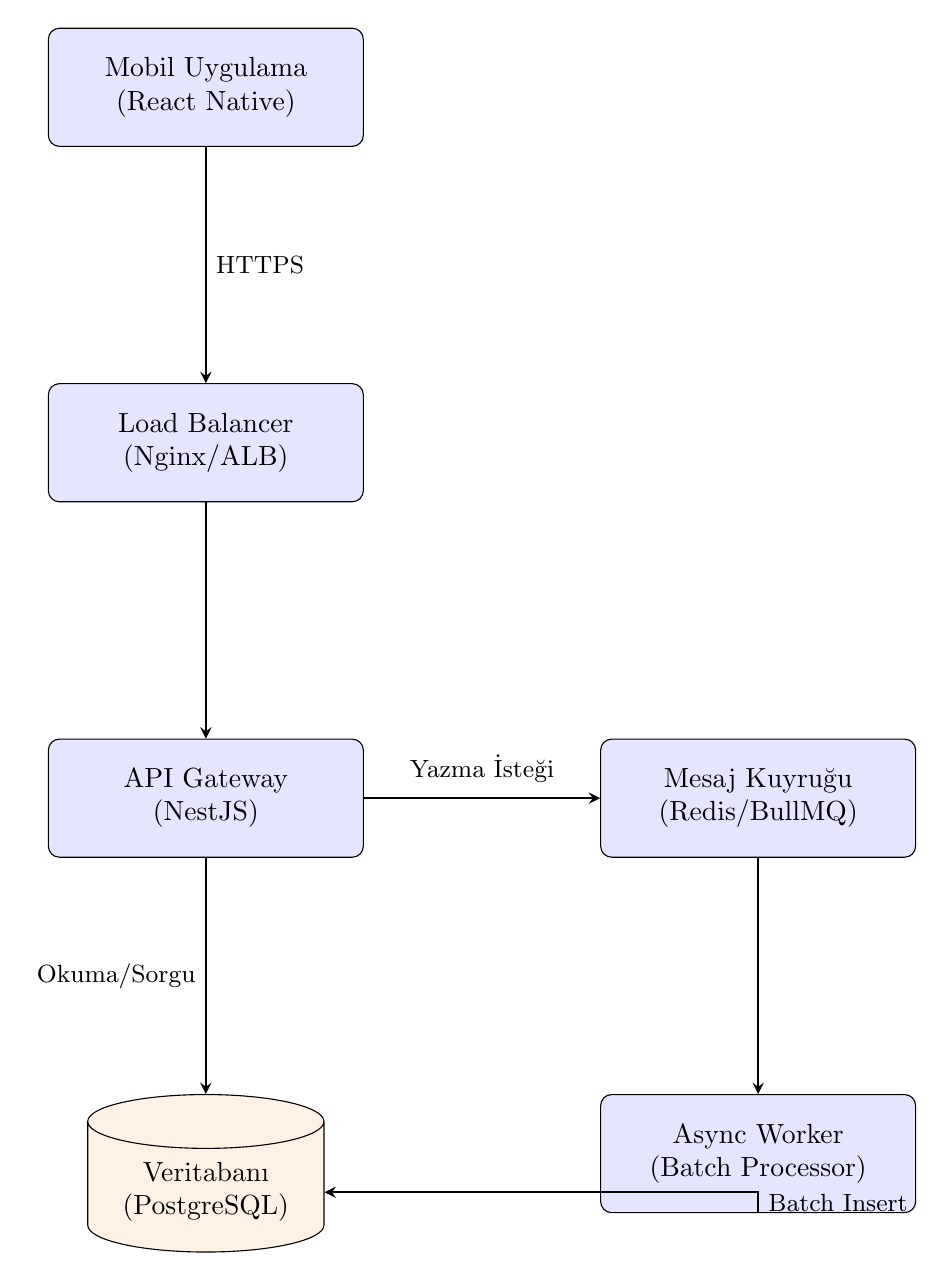
\begin{tikzpicture}[
    node distance=3cm,
    block/.style={rectangle, draw, rounded corners, minimum width=4cm, minimum height=1.5cm, text centered, fill=blue!10, text width=3.5cm},
    db/.style={cylinder, draw, shape border rotate=90, aspect=0.25, minimum width=3cm, minimum height=2cm, text centered, fill=orange!10, text width=2.5cm},
    arrow/.style={thick,->,>=stealth, font=\small}
]

% Nodes
\node (app) [block] {Mobil Uygulama\\(React Native)};
\node (lb) [block, below=of app] {Load Balancer\\(Nginx/ALB)};
\node (api) [block, below=of lb] {API Gateway\\(NestJS)};

% Side branch 
\node (queue) [block, right=of api] {Mesaj Kuyruğu\\(Redis/BullMQ)};
\node (worker) [block, below=of queue] {Async Worker\\(Batch Processor)};

% DB
\node (db) [db, below=of api] {Veritabanı\\(PostgreSQL)};

% Arrows
\draw [arrow] (app) -- node[right] {HTTPS} (lb);
\draw [arrow] (lb) -- (api);
\draw [arrow] (api) -- node[above, yshift=2pt] {Yazma İsteği} (queue);
\draw [arrow] (queue) -- (worker);
\draw [arrow] (worker) |- node[near start, right] {Batch Insert} (db);
\draw [arrow] (api) -- node[left] {Okuma/Sorgu} (db);

\end{tikzpicture}
\caption{Sistem Mimarisi Veri Akış Şeması}
\label{fig:architecture}
\end{figure}

\section{Kullanılan Kritik Algoritmalar}
Uygulamanın zekasını oluşturan algoritmalar, pedagojik, olasılıksal ve güvenlik olmak üzere üç ana başlıkta toplanmıştır.

\subsection{Pedagojik: Aralıklı Tekrar Sistemi (SRS - SM-2)}
Kullanıcının kelime öğrenim sürecini optimize etmek için SuperMemo-2 (SM-2) algoritması temel alınmış ve modern parametrelerle iyileştirilmiştir.

Algoritma, her kelime için bir "Tekrar Aralığı" (Interval - I) ve "Zorluk Faktörü" (Easiness Factor - EF) hesaplar:
\begin{equation}
    EF' = EF + (0.1 - (5 - q) \times (0.08 + (5 - q) \times 0.02))
\end{equation}
Burada $q$, kullanıcının cevabına verdiği kalite puanıdır (0: Hatırlamadım, 5: Mükemmel).
\begin{equation}
    Interval(n) = Interval(n-1) \times EF'
\end{equation}
Bu formül sayesinde, kullanıcı zorlandığı kelimeleri daha sık (örneğin 1 gün sonra), kolay bulduğu kelimeleri daha seyrek (örneğin 15 gün sonra) görerek hafızasını tazeler.

\subsection{Olasılıksal: Ağırlıklı Rastgelelik (Weighted Randomness)}
Loot Box (Ödül Kutusu) sisteminde, her ödülün çıkma ihtimali eşit değildir. Nadir eşyaların ekonomiyi bozmaması için "Kümülatif Ağırlık" algoritması kullanılır.

\textbf{Mantık:}
\begin{enumerate}
    \item Tüm olası ödüllerin ağırlıkları toplanır (Örn: Toplam 1000).
    \item 0 ile 1000 arasında rastgele bir sayı ($R$) üretilir.
    \item Ödüller sırayla gezilir ve ağırlıkları toplanır ($CurrentSum$).
    \item $CurrentSum \geq R$ olduğu andaki ödül seçilir.
\end{enumerate}
Bu yöntem, O(N) karmaşıklığında çalışır ve ödül dağılımını matematiksel olarak kontrol altında tutar.

\subsection{Performans: Sıralama Algoritmaları (Zero-Cost Sort)}
Milyonlarca kullanıcının bulunduğu bir sistemde "Liderlik Tablosu" (Leaderboard) oluşturmak için klasik \texttt{ORDER BY xp DESC} sorgusu çok maliyetlidir. Bunun yerine "Index-Only Scan" stratejisi uygulanmıştır.
Veritabanında \texttt{(cohort\_id, weekly\_xp DESC)} şeklinde oluşturulan B-Tree indeksi, verilerin diskte hali hazırda sıralı tutulmasını sağlar. Böylece sorgu anında herhangi bir sıralama algoritması (Quicksort/Mergesort) çalışmaz, indeks sırayla okunur. Karmaşıklık O(N log N)'den O(1)'e düşürülür (Limitli sorgularda).

\subsection{Güvenlik: Kriptografik Hashleme (Bcrypt)}
Kullanıcı şifreleri, veritabanı sızıntılarına karşı \texttt{bcrypt} algoritması ile korunur.
\begin{itemize}
    \item \textbf{Salting:} Her şifre için rastgele bir "Tuz" (Salt) değeri üretilir.
    \item \textbf{Cost Factor:} İşlemci gücüne göre ayarlanabilir bir zorluk seviyesi (Work Factor - genelde 10 veya 12) belirlenir. Bu, Rainbow Table saldırılarını imkansız kılar.
\end{itemize}

\section{Veritabanı Kümeleme (Clustering) Stratejisi}
Veri modelleme aşamasında, tablolar kullanım desenlerine göre kümeler (Cluster) halinde organize edilmiştir.

\begin{itemize}
    \item \textbf{Content Cluster (Read-Heavy):} Kurslar, Üniteler. Nadiren değişir, çok sık okunur. Redis önbellekleme (Caching) stratejisi bu küme için agresif uygulanır.
    \item \textbf{Activity Cluster (Write-Heavy):} Ders tamamlama logları. \textbf{Partitioning} (Bölümleme) stratejisi ile bu tablo aylık parçalara bölünür (\texttt{lesson\_completions\_2026\_01}). Bu, indeks boyutunu küçültür ve yazma hızını artırır.
    \item \textbf{Economy Cluster (ACID-Critical):} Cüzdan ve Envanter. Veri tutarlılığı her şeyden önemlidir. Transaction izolasyon seviyesi \texttt{READ COMMITTED} veya duruma göre \texttt{SERIALIZABLE} olarak ayarlanır.
\end{itemize}

% -------------------------------------------------------------------
% BÖLÜM 4: UYGULAMA MODÜLLERİ
% -------------------------------------------------------------------
\chapter{Uygulama Modülleri ve Teknik Detaylar}

\section{Kimlik Doğrulama Modülü (AuthModule)}
Güvenlik, uygulamanın temel taşıdır.
\begin{itemize}
    \item \textbf{JWT (JSON Web Token):} Stateless kimlik doğrulama sağlar. Access Token (15 dk) ve Refresh Token (7 gün) stratejisi ile hem güvenlik hem kullanıcı konforu dengelenmiştir.
    \item \textbf{Güvenlik Önlemleri:} Şifreler veritabanında saklanmaz; \texttt{bcrypt} algoritması ile "Salt" eklenerek hashlenir. Rate Limiting ile Brute-Force saldırıları engellenir.
\end{itemize}

\section{Eğitim ve İçerik Yönetimi}
\textbf{Bi Dakika}, hiyerarşik bir içerik yapısına sahiptir: \texttt{Language > Course > Unit > Level > Exercise}.
Bu yapı, PostgreSQL üzerinde "Materialized Path" benzeri sorgu teknikleriyle (Recursive CTEs veya Nested JSON Includes) yönetilerek, kullanıcıya anlık olarak tüm müfredat ağacını sunabilmektedir. Egzersiz içerikleri, esneklik sağlamak amacıyla \textbf{JSONB} formatında saklanır. Bu, ilişkisel veritabanı içinde NoSQL esnekliği sağlar.

\section{Sanal Ekonomi ve Mağaza (Economy Module)}
Uygulama içinde iki para birimi bulunur: \textbf{Kalp (Hearts)} ve \textbf{Elmas (Gems)}.
\subsection{Pessimistic Locking ile Çifte Harcama Önleme}
Eşzamanlı (Concurrent) isteklerde kullanıcının bakiyesinin eksiye düşmemesi için veritabanı seviyesinde kilitleme kullanılır.
\begin{lstlisting}[language=SQL, caption=Pessimistic Locking Örneği]
BEGIN;
SELECT balance FROM user_wallets 
WHERE user_id = 'uuid...' FOR UPDATE; 
-- Bu satır kilitlenir, diğer işlemler bekler.
UPDATE user_wallets SET balance = balance - 500 
WHERE user_id = 'uuid...';
INSERT INTO transactions (...) VALUES (...);
COMMIT;
\end{lstlisting}

\section{Lig ve Rekabet Sistemi}
Kullanıcılar haftalık performanslarına (XP) göre 30 kişilik gruplara (Cohorts) ayrılır.
\begin{itemize}
    \item \textbf{Lazy Allocation:} Lig grupları önceden oluşturulmaz. Kullanıcı o hafta ilk dersini yaptığı an, kendi seviyesindeki (Örn: Gold League) boş bir 30 kişilik odaya (Cohort) yerleştirilir. Bu, inaktif kullanıcıların ligleri doldurmasını engeller.
    \item \textbf{Index-Only Scans:} Liderlik tablosu (Leaderboard) sorguları, sadece indekslerden veri okuyacak şekilde optimize edilmiştir, tabloya disk erişimi yapılmaz.
\end{itemize}

% -------------------------------------------------------------------
% BÖLÜM 5: OPTİMİZASYON VE ÖLÇEKLENEBİLİRLİK
% -------------------------------------------------------------------
\chapter{Optimizasyon ve Ölçeklenebilirlik Stratejileri}

\section{Batch Processing (Toplu İşleme)}
\textit{Bi Dakika}, milyonlarca kullanıcının aynı anda ders bitirdiği senaryolara hazırlıklıdır. Her ders bitiminde veritabanına doğrudan yazmak yerine (Synchronous Write), bu veriler önce yüksek hızlı bir bellek içi kuyruğa (Redis/BullMQ) atılır.
Arka planda çalışan "Worker" sunucular, bu kuyruktaki verileri 1000'erli paketler halinde (Batch) alarak veritabanına tek bir sorguda yazar (\texttt{INSERT INTO ... VALUES (...), (...)}). Bu yöntem, veritabanı yükünü %90 oranında azaltır.

\section{Veritabanı Partitioning}
Zamanla milyarlarca satıra ulaşabilecek log tabloları (\texttt{lesson\_completions}, \texttt{transaction\_history}), tarih bazlı (Range Partitioning) parçalara ayrılmıştır. Örneğin, 2026 Ocak verileri ile 2026 Şubat verileri disk üzerinde farklı dosyalarda tutulur. Bu, eski verilere erişimin nadir olduğu durumlarda sorgu performansını korur ve arşivlemeyi kolaylaştırır.

\section{GIN Indexing}
JSONB formatında saklanan egzersiz içerikleri (soru metni, seçenekler) üzerinde full-text search yapabilmek için GIN (Generalized Inverted Index) kullanılmıştır. Bu, JSON verisi içinde geçen herhangi bir kelimeye milisaniyeler içinde ulaşmayı mümkün kılar.

% -------------------------------------------------------------------
% BÖLÜM 6: SONUÇ
% -------------------------------------------------------------------
\chapter{Sonuç ve Gelecek Çalışmalar}

\section{Proje Kazanımları}
Bu bitirme çalışması sonucunda;
\begin{enumerate}
    \item \textbf{Pazara Hazır Ürün:} Sadece bir prototip değil, App Store ve Play Store'a yüklenebilecek olgunlukta (Production-ready) bir ürün ortaya çıkmıştır.
    \item \textbf{Mimari Yetkinlik:} NestJS, PostgreSQL ve React Native gibi modern teknolojilerin en iyi uygulama pratikleri (Best Practices) ile nasıl entegre edileceği gösterilmiştir.
    \item \textbf{Özgün Değer:} "Bi Dakika" konsepti ile mikro-öğrenme alanında özgün bir kullanıcı deneyimi tasarlanmıştır.
\end{enumerate}

\section{Gelecek Planları}
Projenin sonraki sürümleri için planlanan özellikler:
\begin{itemize}
    \item \textbf{AI Destekli Konuşma Pratiği:} OpenAI Whisper veya benzeri modellerle kullanıcının telaffuzunun analiz edilmesi.
    \item \textbf{Çoklu Oyunculu (Multiplayer) Mod:} Kullanıcıların anlık olarak birbirleriyle kelime düellosu yapabilmesi.
    \item \textbf{Çevrimdışı (Offline) Mod:} İnternet olmadan da ders yapabilme yeteneğinin tam kapsamlı hale getirilmesi.
\end{itemize}

% -------------------------------------------------------------------
% KAYNAKÇA
% -------------------------------------------------------------------
\begin{thebibliography}{9}

\bibitem{deterding}
Deterding, S., Dixon, D., Khaled, R., \& Nacke, L. (2011). 
\textit{From game design elements to gamefulness: defining gamification}. 
In Proceedings of the 15th international academic MindTrek conference (pp. 9-15).

\bibitem{miller}
Miller, G. A. (1956). 
\textit{The magical number seven, plus or minus two: Some limits on our capacity for processing information}. 
Psychological review, 63(2), 81.

\bibitem{wozniak}
Wozniak, P. A. (1990). 
\textit{Optimization of learning}. 
Master's Thesis, University of Technology in Poznan. (SM-2 Algorithm Source).

\bibitem{nestjs}
NestJS Documentation. 
\textit{https://docs.nestjs.com/}. 
Erişim Tarihi: 2025.

\bibitem{reactnative}
React Native Documentation. 
\textit{https://reactnative.dev/}. 
Erişim Tarihi: 2025.

\bibitem{postgresql}
PostgreSQL 16 Documentation. 
\textit{Partitioning and High Availability}. 
Erişim Tarihi: 2025.

\end{thebibliography}

\end{document}
